\chapter{EXPERIMENTO}
\label{chap:experimento}

Para aplicar os conceitos vistos na seção \ref{chap:estudo}, foi proposto um desafio em que consiste em modelar um experimento contendo um helicóptero de papel. O objetivo deste desafio é observar como a saída desejada, neste caso o maior tempo de voo, está relacionada com as variáveis de entrada.  

Para conceber o protótipo do helicóptero para o estudo, foi utilizado o modelo proposto pela metodologia \textit{SixSigma}, conforme visto na Figura \ref{fig:model_heli}. 

\begin{figure}[H]
  \caption{Modelo do helicóptero de papel.}
  \centering
  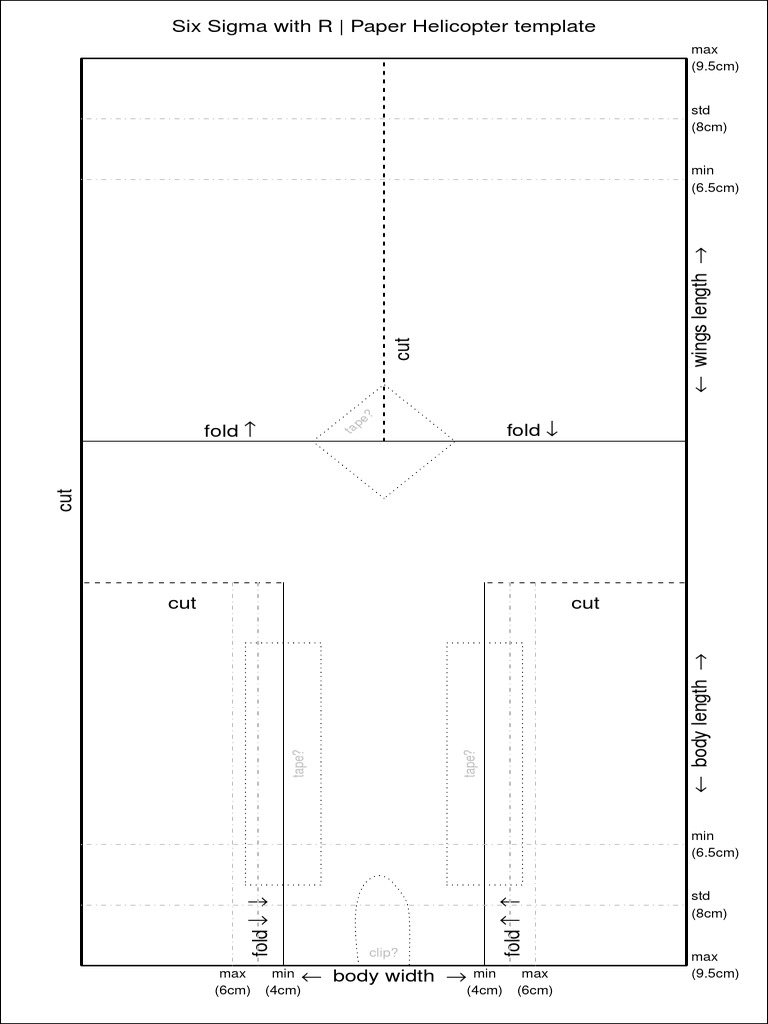
\includegraphics[width=0.7\textwidth]{images/helicopter.jpeg}
  \label{fig:model_heli}
\end{figure}

Seguindo as recomendações do \textit{template}, foi obtido como modelo de configuração inicial, o helicóptero visto na Figura \ref{fig:heli_papel}. Este, apresenta as asas e o corpo com o comprimento máximo (9,5 cm), e que não deverá ser alterado. O seu tempo de voo é medido desde o momento em que é lançado da altura definida até o momento em que o mesmo atinge o solo.

% O tempo de voo é medido desde o momento em que o helicóptero é lançado da altura definida até o momento em que atinge o solo.    

% Após as dobras e cortes recomendados pelo \textit{template}, o protótipo obtido como configuração inicial para análise do estudo pode ser visto na Figura \ref{fig:heli_papel}.

\begin{figure}[H]
  \caption{Helicóptero de papel.}
  \centering
  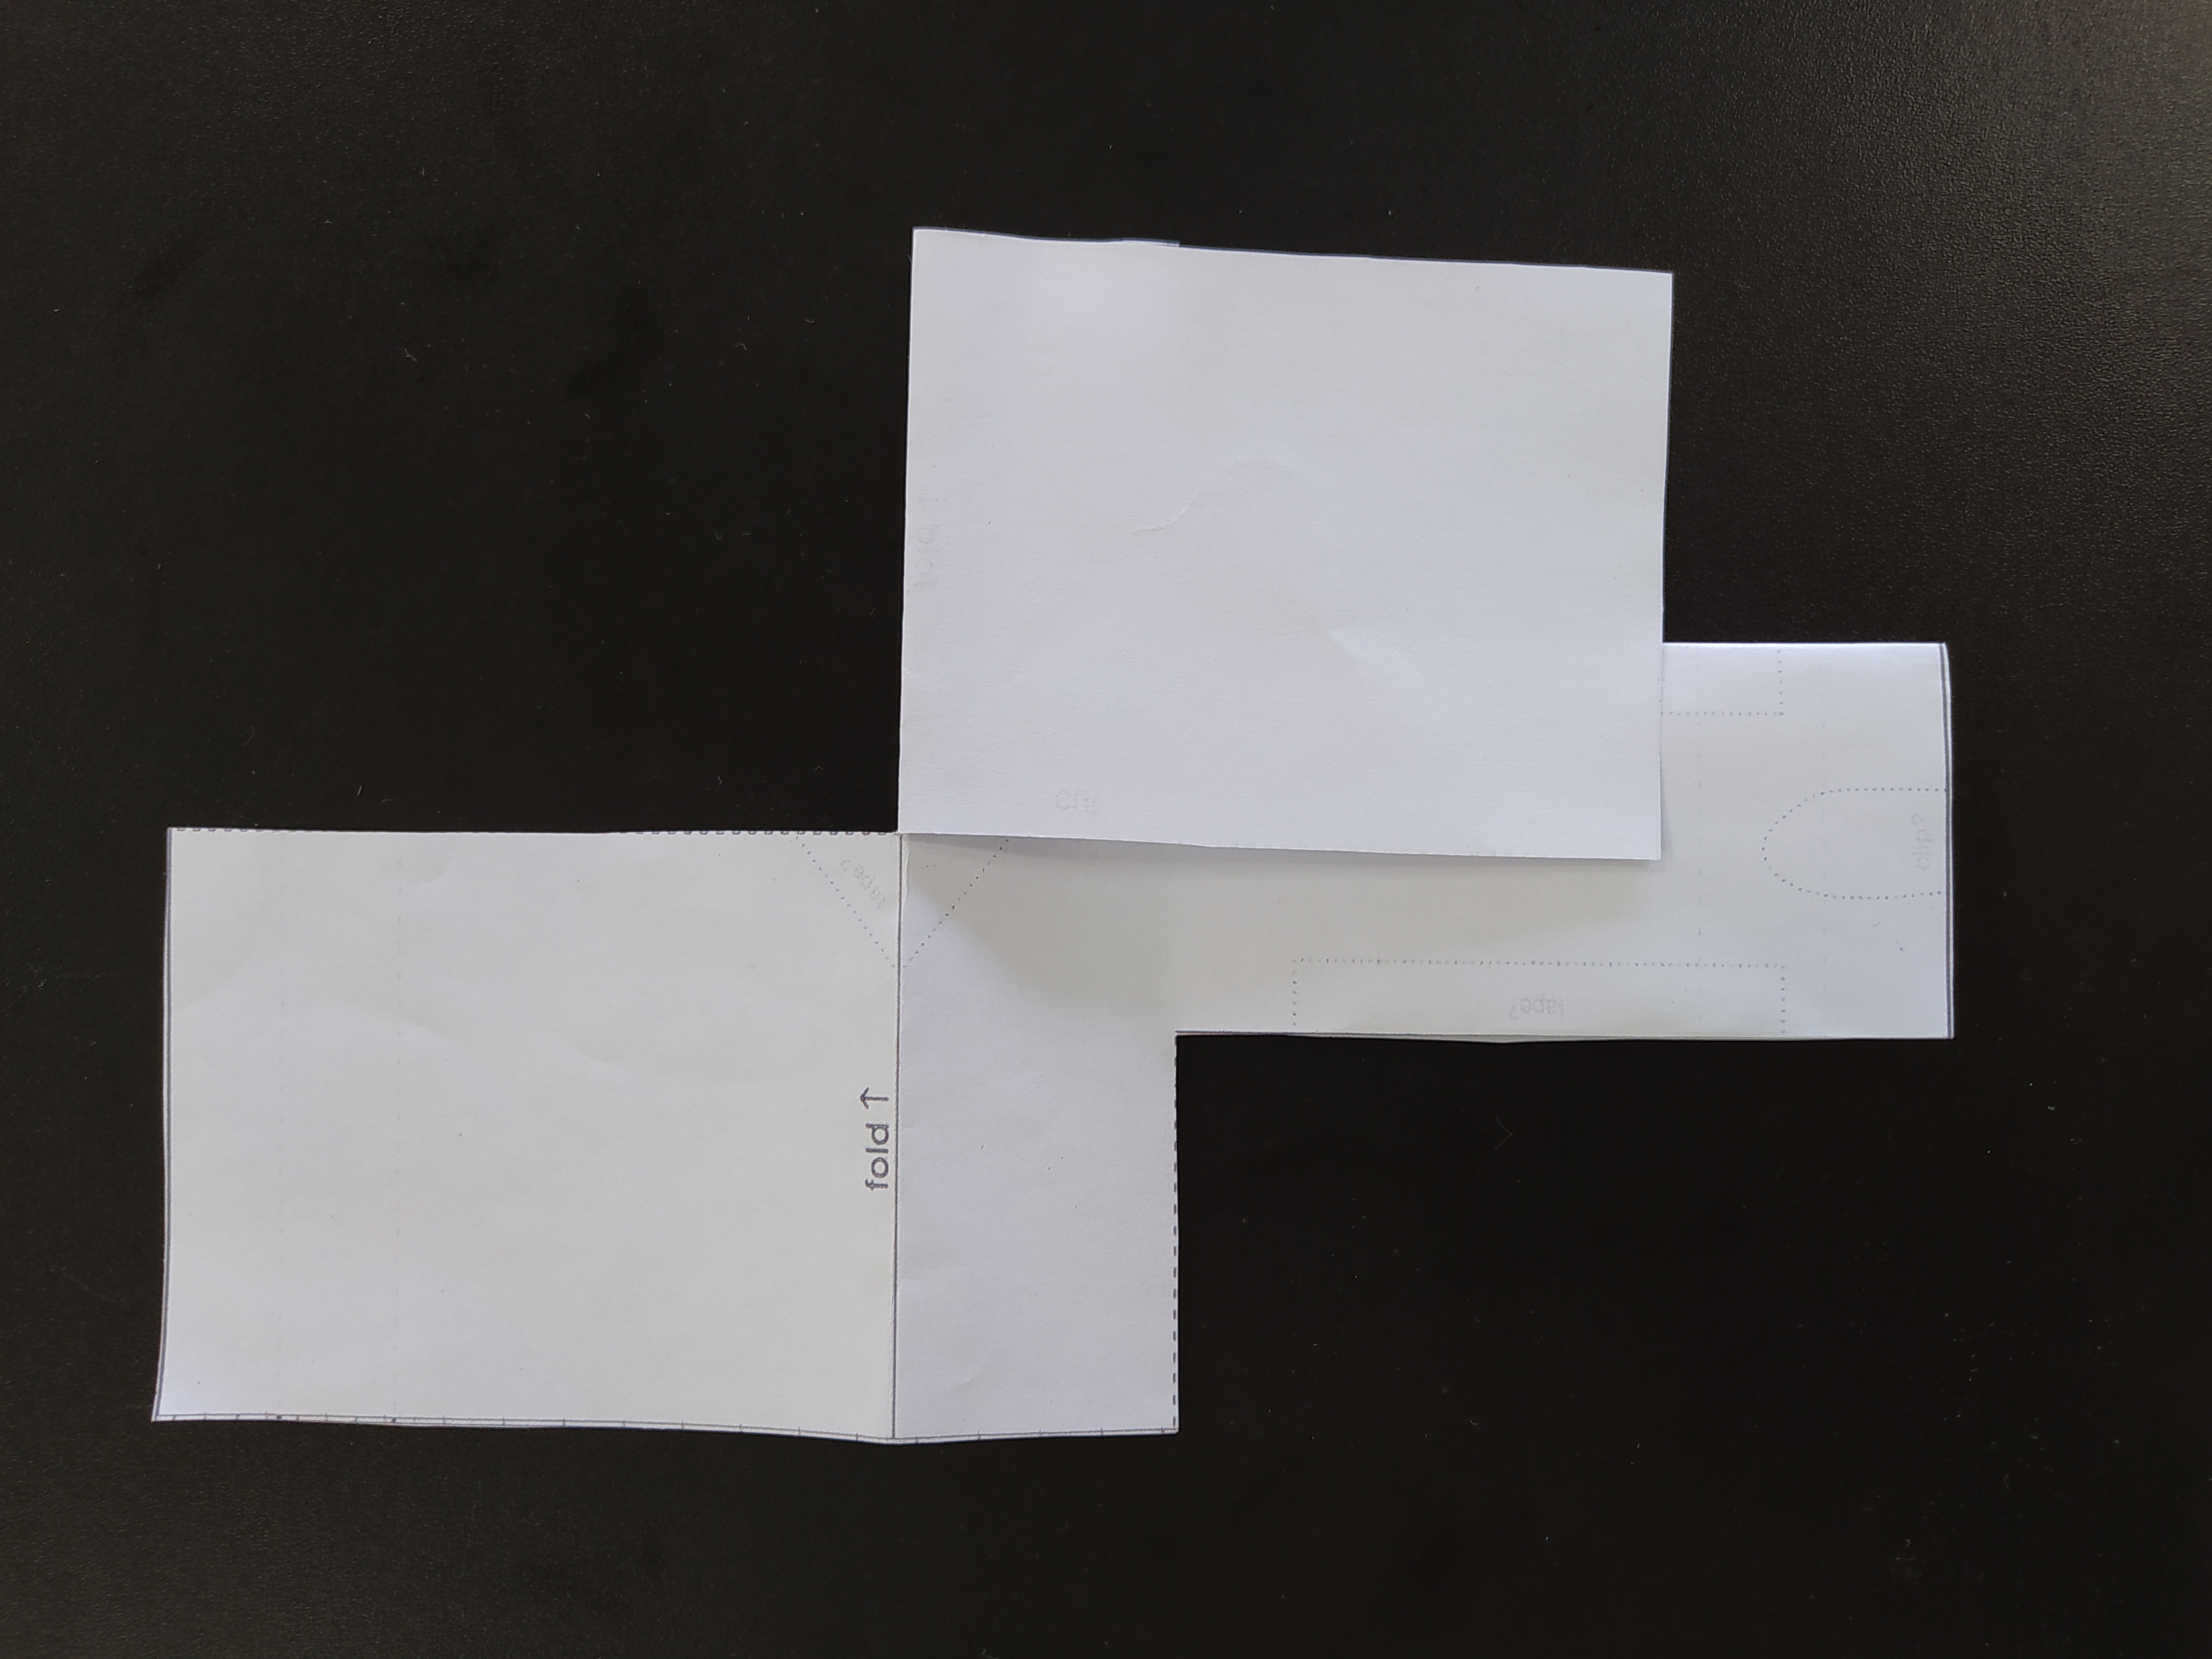
\includegraphics[angle=0,width=1\textwidth]{images/IMG_20200918_162251.jpg}
  \caption*{Fonte: Autoria própria.}
  \label{fig:heli_papel}
\end{figure}

Para realizar os testes, foram considerados alguns fatores que influenciam no tempo de voo, conforme vistos na Tabela \ref{tab:fatores}.

\begin{table}[H]
  \caption{Fatores considerados para alterar a estrutura.}
  \centering
  \begin{tabular}{|c|c|c|}
  \hline
  \rowcolor[HTML]{EFEFEF} 
  \textbf{Fatores}              & \textbf{Configuração atual} & \textbf{Alteração permitida} \\ \hline
  Comprimento (asa e corpo) (m) & 0,095                       & Não                          \\ \hline
  \rowcolor[HTML]{EFEFEF} 
  Clipe                         & Não                         & Sim                          \\ \hline
  \rowcolor[HTML]{FFFFFF} 
  Altura (m)                    & 1,30                        & 2,10                         \\ \hline
  \rowcolor[HTML]{EFEFEF} 
  Adesivo (Asa)                 & Não                         & Sim                          \\ \hline
  \rowcolor[HTML]{FFFFFF} 
  Adesivo (Corpo/Esquerdo)         & Não                         & Sim                          \\ \hline
  \rowcolor[HTML]{EFEFEF} 
  Adesivo (Corpo/Direito)          & Não                         & Sim                          \\ \hline
  \end{tabular}
  \caption*{Fonte: Autoria própria.}
  \label{tab:fatores}
  \end{table}

Por fim, foi construída a Tabela \ref{tab:dados_experimento} que contém o tempo de voo para cada uma das possíveis combinações dos fatores. Para as variáveis \textit{clipe}, \textit{Ad\_top}, \textit{Ad\_esquerda} e \textit{Ad\_direita} o simbolo ``\textbf{+}'' indica a sua presença enquanto o ``\textbf{-}'' representa a sua ausência, já para a variável \textit{Altura} o ``\textbf{+}'' retrata sua configuração inicial de 1,30 metros e o ``\textbf{-}'' representa a altura de 2,10 metros. O próximo passo é utilizar a ferramenta R para realizar o estudo de planejamento de experimentos (DOE) e analisar qual das configurações está exercendo uma maior influência no experimento, que será discutido na seção \ref{chap:resultados}.



\begin{table}[H]
  \centering
  \caption{Dados do experimento.}
  \begin{tabular}{|c|c|c|c|c|c|}
  \hline
  \rowcolor[HTML]{EFEFEF} 
  \textbf{Altura}           & \textbf{Clipe}            & \textbf{Ad\_top}          & \textbf{Ad\_esquerda}     & \textbf{Ad\_direita} & \textbf{Tempo}               \\ \hline
  \rowcolor[HTML]{FFFFFF} 
  -                         & -                         & -                         & -                         & -                    & 1,27                         \\ \hline
  \rowcolor[HTML]{EFEFEF} 
  +                         & -                         & -                         & -                         & -                    & 1,27                         \\ \hline
  \rowcolor[HTML]{FFFFFF} 
  -                         & +                         & -                         & -                         & -                    & 1,10                         \\ \hline
  \rowcolor[HTML]{EFEFEF} 
  +                         & +                         & -                         & -                         & -                    & 1,70                         \\ \hline
  \rowcolor[HTML]{FFFFFF} 
  -                         & -                         & +                         & -                         & -                    & 1,31                         \\ \hline
  \rowcolor[HTML]{EFEFEF} 
  +                         & -                         & +                         & -                         & -                    & 1,82                         \\ \hline
  \rowcolor[HTML]{FFFFFF} 
  -                         & +                         & +                         & -                         & -                    & 1,30                         \\ \hline
  \rowcolor[HTML]{EFEFEF} 
  +                         & +                         & +                         & -                         & -                    & 1,75                         \\ \hline
  \rowcolor[HTML]{FFFFFF} 
  -                         & -                         & -                         & +                         & -                    & 1,36                         \\ \hline
  \rowcolor[HTML]{EFEFEF} 
  +                         & -                         & -                         & +                         & -                    & 1,92                         \\ \hline
  \rowcolor[HTML]{FFFFFF} 
  -                         & +                         & -                         & +                         & -                    & 1,52                         \\ \hline
  \rowcolor[HTML]{EFEFEF} 
  +                         & +                         & -                         & +                         & -                    & 1,71                         \\ \hline
  \rowcolor[HTML]{FFFFFF} 
  -                         & -                         & +                         & +                         & -                    & 1,40                         \\ \hline
  \rowcolor[HTML]{EFEFEF} 
  +                         & -                         & +                         & +                         & -                    & 1,83                         \\ \hline
  \rowcolor[HTML]{FFFFFF} 
  -                         & +                         & +                         & +                         & -                    & 1,32                         \\ \hline
  \rowcolor[HTML]{EFEFEF} 
  +                         & +                         & +                         & +                         & -                    & 1,74                         \\ \hline
  \rowcolor[HTML]{FFFFFF} 
  -                         & -                         & -                         & -                         & +                    & 1,50                         \\ \hline
  \rowcolor[HTML]{EFEFEF} 
  +                         & -                         & -                         & -                         & +                    & 1,91                         \\ \hline
  \rowcolor[HTML]{FFFFFF} 
  -                         & +                         & -                         & -                         & +                    & 1,23                         \\ \hline
  \rowcolor[HTML]{EFEFEF} 
  +                         & +                         & -                         & -                         & +                    & 1,55                         \\ \hline
  \rowcolor[HTML]{FFFFFF} 
  -                         & -                         & +                         & -                         & +                    & 1,42                         \\ \hline
  \rowcolor[HTML]{EFEFEF} 
  \cellcolor[HTML]{EFEFEF}+ & -                         & \cellcolor[HTML]{EFEFEF}+ & -                         & +                    & 2,04                         \\ \hline
  \rowcolor[HTML]{FFFFFF} 
  -                         & +                         & +                         & -                         & +                    & 1,35                         \\ \hline
  \rowcolor[HTML]{EFEFEF} 
  +                         & +                         & +                         & \cellcolor[HTML]{EFEFEF}- & +                    & \cellcolor[HTML]{EFEFEF}1,68 \\ \hline
  \rowcolor[HTML]{FFFFFF} 
  -                         & -                         & -                         & +                         & +                    & 1,44                         \\ \hline
  \rowcolor[HTML]{EFEFEF} 
  +                         & \cellcolor[HTML]{EFEFEF}- & \cellcolor[HTML]{EFEFEF}- & +                         & +                    & \cellcolor[HTML]{EFEFEF}1,58 \\ \hline
  \rowcolor[HTML]{FFFFFF} 
  -                         & +                         & -                         & +                         & +                    & 1,25                         \\ \hline
  \rowcolor[HTML]{EFEFEF} 
  +                         & +                         & \cellcolor[HTML]{EFEFEF}- & +                         & +                    & \cellcolor[HTML]{EFEFEF}1,73 \\ \hline
  \rowcolor[HTML]{FFFFFF} 
  -                         & -                         & +                         & +                         & +                    & 1,32                         \\ \hline
  \rowcolor[HTML]{EFEFEF} 
  +                         & \cellcolor[HTML]{EFEFEF}- & +                         & +                         & +                    & \cellcolor[HTML]{EFEFEF}1,86 \\ \hline
  \rowcolor[HTML]{FFFFFF} 
  -                         & +                         & +                         & +                         & +                    & 1,17                         \\ \hline
  \rowcolor[HTML]{EFEFEF} 
  +                         & +                         & +                         & +                         & +                    & 1,63                         \\ \hline
  \end{tabular}
  \label{tab:dados_experimento}
  \caption*{Fonte: Autoria própria.}
  \end{table}

